\documentclass{article}
\usepackage{xcolor, graphicx}
\usepackage{mathabx}
\usepackage{subcaption}
\usepackage{hyperref}
\hypersetup{colorlinks=false}
\author{Edderic Ugaddan}
\title{Granuvolver}
\begin{document}
	\maketitle
	\tableofcontents
	\section{Gratitude}

		Special thanks goes to Dr. Benjamin Broening and Dr. Barry Lawson. First of all, thank you for being wonderful top-notch professors. I've really enjoyed all my classes with you, learning from you, and having one-on-ones with you, no matter how stressful it was at times. Thank you for helping me create my interdisciplinary major, Computer Music, and taking me under your wings as an advisee, giving me advice and showing me a different way to look at things whenever I was getting too caught up with an idea.  In the end, I feel that I've become a much better programmer, musician, and most of all, person.

	\section{Introduction}

		The objective of this Computer Music interdisciplinary senior thesis is to explore the combination of Granular Synthesis and Convolution. This entails programming a custom-made Max for Live (M4L) MIDI instrument that combines the two technologies, analyzing the sounds that come out of this combination, and finally creating music using the resulting sounds as source material. Granular synthesis is the method of producing interesting, texturally rich sounds by overlaying grains, sets of samples that are about 100 ms. or less in length. Convolution describes the mathematical process of sliding multiplication of two signals.   To the knowledge of the author, no MIDI instrument has been made that is specifically made only for exploring the combining of these two technologies.

		\begin{figure}[h!]
		  \centering
		  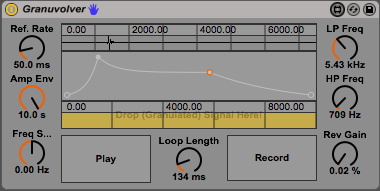
\includegraphics[width=1\textwidth]{images/Granuvolver}
		  \caption{Granuvolver}
		\end{figure}

	\section{Granular Synthesis}
		\subsection{What is it?}
			Granular Synthesis is the creation of sound via means of aggregating various sets of samples called grains. A grain is defined as:
			\begin{quote} 
				\ldots a brief microacoustic event, with a duration near the threshold of human auditory perception, typically \ldots [being less than] one tenth of a second, serving as a building block for sound objects.\cite[Loc. 1024]{Curtis_gs_def} 
			\end{quote}

			It was largely inaccessible in the past due to technological limitations of analog circuitry and tape. However, thanks to the advances in computing and hardware, composers are now able to digitalize audio and work with the latter in a sample-by-sample basis, thereby letting composers explore the "extreme limits of perception and performance."\cite[Loc. 334]{Curtis_gs}  Combining these grains helps us create animated, texturally rich sonic atmospheres.\cite[Loc. 1024]{Curtis_gs_def}    
			
	\section{Convolution}
		\subsection{What is it?}
			Convolution, in digital signal processing, is the mathematical process of sliding and overlapping two signals together, point-wise multiplying the coefficients, and summing the products. In more mathematically-precise terms, 

		\begin{equation}
			(f \convolution g) = \sum_{m=-\infty}^{\infty} f[m] g[n-m] 
		\end{equation} 
		where $f$ and $g$ are the two signals being convolved.\cite[pp. 121]{JOS_conv}. $m$ can represent time in samples.

		\subsection{Reverberation}

			Convolution, amongst music producers, is most famous for simulating the reverberation of physical spaces by a sound object.  For example, consider recording a drum that is hit in a small room, and then recording the reverberation of a large concert hall (stimulated by a quick transient such as a loud clap).  Convolving the two signals results in a "smearing"; the transient of the drum hit is smeared by the long reverb tail of the concert hall. The acoustical result would sound as if the drum hit was played in the large concert hall.

		\subsection{Algorithmic Efficiency}

			The naive implementation, which is called "direct" convolution, has a time efficiency of $O(n^2)$, where $n$ is the number of samples. This is terribly inefficient, considering that $n$ is quite large even for a small amount of time--the standard CD-quality audio signal has a sampling rate of 44.1 kHz (three seconds of recording, for example, would amount to greater than $10^5$ samples, and the resulting floating-point operations for convolution would be in the order of $10^{10}$).  

			Performing the Fast Fourier Transform (FFT), the point-wise multiplication, and the accompanying inverse FFT of the two signals shaves the time complexity to $O(n$log$n)$. A \emph{drastic} improvement indeed.  However, since $n$ is quite large, the convolution will still incur lots of latency and thus cannot be considered "real-time."  More complicated FFT algorithms take advantage of the audio signals' \emph{linearity} to speed up the convolution process. Partitioning the signals and doing many smaller FFTs in parallel helps decrease latency to the point of making it usable for real-time convolution.\cite{Batten_conv} Dr. Alex Harker's real-time implementation, called $multiconvolve$\~{}, is a Max/MSP object that is used in this thesis to help speed up the music making process.\cite{pa}


	\section{Granuvolver}
		\subsection{Why Max?}
		Granuvolver was originally made using the cross-platform Virtual Studio Effect (VST) SDK using C++. VST, developed by Steinberg, Inc. is a very popular audio plugin format that is supported by major Digital Audio Workstations (DAWs), such as Logic, Ableton Live, Cubase, ProTools, and Reaper.  Unfortunately, implementing VSTs is not trivial. VST SDKs do not come with built-in audio effects or GUI elements. Also one can easily get stuck working more on IDE configuration settings than on actual programming. See section on  \href{http://teragonaudio.com/article/How-to-make-VST-plugins-in-Visual-Studio.html}{build settings for Visual Studio}, for example.

		Max, a proprietary software developed by Cycling 74, is a graphical, programmable, patching environment written in C.  Objects have inlets and outlets that one can connect to other objects. One can create more powerful objects by making one that is composed of many built-in objects. One can also create external objects in Javascript and Java very easily. However, if one wants more efficient performance and does not mind doing manual garbage collection, one can even develop externals in pure C, C++, and even in Objective-C. Unfortunately, a regular undiscounted license is a hefty \$399.

		Yet, Max ultimately became the final implementation environment solely for several reasons. First, it allows fast prototyping. Max (vers. 6.1) has over 1,000 native objects that can be quickly used, such as objects for dropping (and recognizing paths) of audio files, displaying waveforms and selecting sections of the waveforms, and filtering an incoming audio signal. By providing easily editable and usable GUI elements and providing DSP objects, one can really put more time into actual music production and less into development. Second, users can develop Max for Live (M4L) objects, which can be easily and seamlessly patched, edited, and used within powerful Ableton Live 9 software for further editing and processing.
		\subsection{Features}

			\begin{enumerate}
				\item Stereo-based granulation of audio signals.
				\item Granulator uses Gaussian Normal Distribution with editable mean and pseudo-width to stochastically pick the next area to iterate.
				\item Polyphonic (up to 3 simultaneous voices).
				\item Subtractive synthesis (using a combo of low-pass and high-pass filters)
				\item Slope of curves of amplitude envelope are editable.
				\item Granulation of a signal can then be recorded into buffer to be used for real-time convolution of the granulated signals.

			\end{enumerate}
		\subsection{Installation}
			\subsubsection{OSX 64-bit}
				Granuvolver has been tested on OSX 10.7.5 Lion using Ableton Suite 9.0.6 and Max 6.1.1 64-bit. It should work on Ableton Live 9.0+ as well, as long as the user has Max for Live plugin installed. 

				\begin{enumerate}
				\item Open Max 6.1.1. Place Granuvolver.amxd along with its subpatches (ones ending in \emph{.maxpat}) in the search path of Max. While at the menu bar, select \emph{Options} and \emph{File Preferences}.  Press the \emph{+} button (in the bottom left corner) to add the Granuvolver folder. See Figure~\ref{installation_figure} on page~\pageref{installation_figure}.

				\begin{figure}[h!]
				  \centering
			    \includegraphics[width=1\textwidth]{images/Installation}
				  \caption{Added the Granuvolver folder to the search path}
				  \label{installation_figure}
				\end{figure}

				\item Open a new (or existing) project by Ableton Live (or Suite) 9 and place \emph{Granuvolver.amxd} onto a MIDI track. See Figure~\ref{Ableton_MIDI_Granuvolver} on page~\pageref{Ableton_MIDI_Granuvolver}.

				\begin{figure}[h!]
				  \centering
			    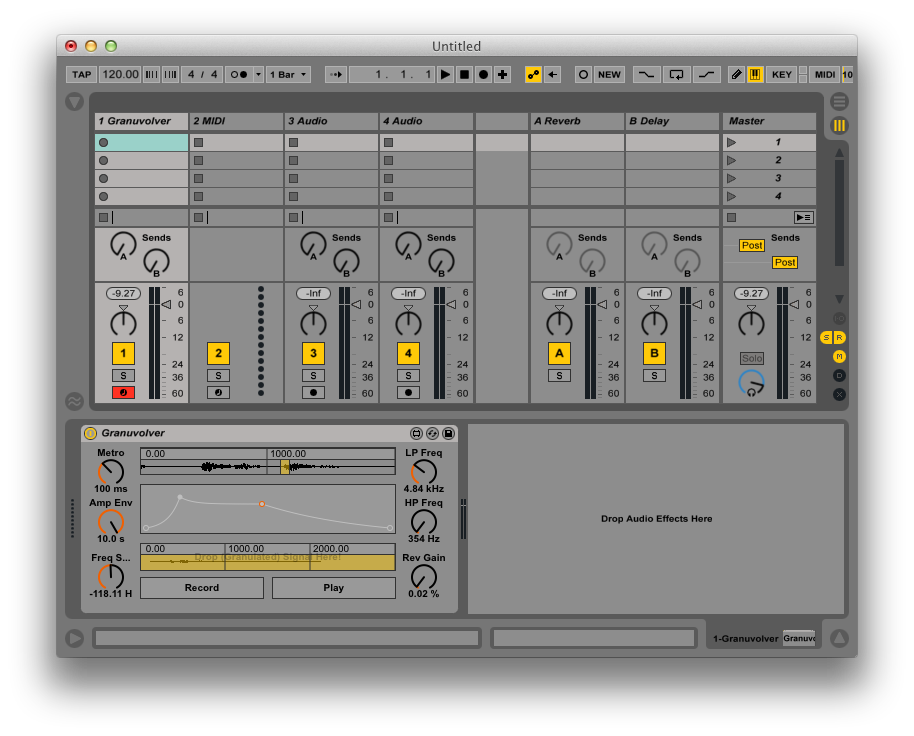
\includegraphics[width=1\textwidth]{images/ableton}
				  \caption{Added Granuvolver to a MIDI track}
					\label{Ableton_MIDI_Granuvolver}.
				\end{figure}

				\end{enumerate}

		\subsection{How to use}
			\begin{enumerate}
				\item Drag a \emph{stereo} (2-channel) recording onto the waveform object on the top-center third half. Stereo (as opposed to mono) for version 1 is a must--mono causes the granulator to only play the left channel. After doing so, the waveform will only show the left channel in order to save screen space. See Figure~\ref{add_2_channel_audio_to_granulate} on page~\pageref{add_2_channel_audio_to_granulate}.
				If a stereo audio file is not available, user can record one. Make sure \emph{I.O} at the right-hand side is selected (yellow). Use an Audio track, and make sure to select \emph{Ext. In 1/2} as \emph{Audio From}. Start recording by pressing a row's circle button right underneath the track name.  See Figures~\ref{about_to_record_stereo} and \ref{recording_stereo} on page~\pageref{recording a stereo signal}.

				\begin{figure}[h!]
				  \centering
			    \includegraphics[width=0.75\textwidth]{images/granulator_waveform_fresh}
				  \caption{Added a 2-channel audio signal onto the top-center waveform area to be granulated}
				  \label{add_2_channel_audio_to_granulate}
				\end{figure}

				\begin{figure}[h!]
				  \centering
					\begin{subfigure}[b]{0.5\textwidth}
				    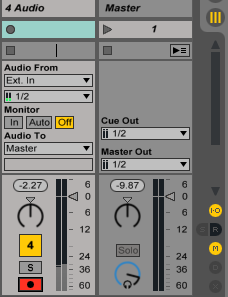
\includegraphics[width=\textwidth]{images/about_to_record_stereo}
					  \caption{Setting up}
					  \label{about_to_record_stereo}
					\end{subfigure}
					\qquad
					\begin{subfigure}[b]{0.3\textwidth}
				    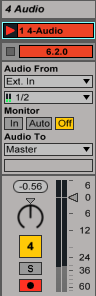
\includegraphics[width=\textwidth]{images/recording_stereo}
					  \caption{Recording into a clip}
					  \label{recording_stereo}
					\end{subfigure}
					\caption{Recording a stereo signal}
					\label{recording a stereo signal}
				\end{figure}

				\item Play MIDI notes. You should hear the waveform. The waveform should be transposed depending on the note pressed.  

				\item Click and drag on the waveform with an up movement. This section by default is the \emph{stochastic iterator range selector}. Doing so activates the Gaussian Normal pseudo-random generator. The middle of the left and right bounds of the yellow area is the mean of the Gaussian. Thus, the larger the area covered by yellow, the more "random" it should sound.  You should hear stuttering in stereo.  Select a range for the granulator to stochastically iterate by dragging the selection left or right. See Figure~\ref{selected_stochastic_loop_area} on page~\pageref{selected_stochastic_loop_area}.

				\item Adjust the \emph{loop length} dial to change loop length to suit your needs.

				\item Play around with the \emph{metro} dial.  This parameter affects how quickly the Gaussian Pseudo-Random generator outputs a number that influences the section of sound to iterate.  The shorter it is, the faster the change, and vice versa.

				\item Play with the \emph{amp env} dial. This dial influences the length of the amplitude envelope.  Once you like the length, you could further customize the changes in amplitude by editing the amplitude envelope.  

				\item Amplitude envelope, by default, is given an Attack-Sustain-Decay-Release (ADSR) envelope. X-coordinates represent time, starting when a note is pressed, while Y-coordinates represent amplitude over that period of time.  The orange dot is the Sustain dot.  Make sure to only have one sustain.  You may add white dots (representing other non-sustain ones), as many as you wish if you'd like a more complicated amplitude modulation. You could remove the extra white dots by focusing the cursor to one, holding down \emph{SHIFT}, and then pressing on the dot.  You could also change the steepness of slopes by holding down \emph{ALT} and clicking and dragging up or down on the curve of interest, depending on how steep you want the curve to be.  See Figures~\ref{amp_env_more_points} and \ref{amp_env_change_slopes} on page~\pageref{editing amplitude envelope}.

				\item Play around with other dials like the Freq. Shift (Frequency Shifter) and the Low Pass and High Pass Frequency knobs to further change the sound to your liking.

				\item Press down \emph{Record} to record a signal that is being granulated. The recording can be up to about 3 seconds.

				\item Adjust the \emph{Rev. Gain} (Reverb Gain) accordingly and adore the lush sounds that come out of \emph{Granuvolver}.  Careful with the gain as gain spikes from the convolution might occur, depending on frequencies present in the convolution--some frequencies might get too resonant and "blow up," causing some undesirable clipping.

			
				\begin{figure}[h!]
				  \centering
			    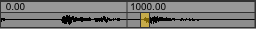
\includegraphics[width=0.75\textwidth]{images/granulator_waveform_selected}
				  \caption{Selected stochastic loop area}
				  \label{selected_stochastic_loop_area}
				\end{figure}


				\begin{figure}[h!]
				  \centering
					\begin{subfigure}[b]{0.5\textwidth}
				    
\includegraphics[width=\textwidth]{images/amp_env_more_points}
					  \caption{Adding new points}
					  \label{amp_env_more_points}
					\end{subfigure}
					\qquad
					\begin{subfigure}[b]{0.5\textwidth}
				    
\includegraphics[width=\textwidth]{images/amp_env_change_slopes}
					  \caption{Changing slope of curves}
					  \label{amp_env_change_slopes}
					\end{subfigure}
					\caption{Editing amplitude envelope}
					\label{editing amplitude envelope}
				\end{figure}


			\end{enumerate}

		


		\subsection{Future Improvements}
			\subsubsection{Known Bugs}
				\begin{enumerate}
					\item Dropping a mono audio file into the waveform for the granulator results in the granulator only playing audio in the left channel.

					\item Loading another instance of Granuvolver is a problem since the \emph{buffer}\~{} objects in each Granuvolver are not given names that are unique to each Granuvolver instance.  Therefore, dropping one audio file to be granulated in one instance will store the audio in other instances as well.

					\item Convolution recording is not being saved.  Therefore, attempting to save the Live Set (even doing \emph{Collect all and save}) and restarting Ableton Live does no good in saving a recording that was recorded via \emph{Record} button.

					\item Start and end points of the granulator \emph{waveform}\~{} selection are also not saved just like in the case above.

					\item Information relating to the Amplitude Envelope \emph{function}\~{} object, such as $X,Y,$ and $curve$, is not being stored in saving the Ableton Live Set. 

				\end{enumerate}

				Further progress can be found at \href{https://www.pivotaltracker.com/s/projects/961764}{Granuvolver's Pivotal Tracker site.}

			\subsubsection{Suggested Improvements}
				\begin{enumerate}
					\item Develop a bypass button for \emph{reverb gain}.
					
					\item Be able to adjust the number of voices dynamically in order to save CPU cycles.
					
					\item Make use of the \emph{polybuffer}\~{} object in order to load a folder of samples to quickly play around with.  This is faster than manually dragging-and-dropping each audio file to be granulated.


				\end{enumerate}
	\section{Music Piece}
		"Elements" is a short piece that was only made using three sampled audio files--one of water dripping $W$, starting a fire $F$, and a burst of thunder $T$. The general idea was to granulate each of those signals and use them as the Impulse Response (IR) for convolution. Once recorded, another signal is granulated live, and is also convolved with the recorded granulated signal live. Different combinations were used for the live granulated signal and the IR: $(F,F), (W,W), (L,L), (F,W)$, etc. Most of the settings used long amplitude envelopes (high amp. env.), high reverb gain, and long recordings of the granulated signals for long reverb tails, resulting in sonically rich textures.

		The audio file can be found at \href{https://soundcloud.com/edderic/elements}{Soundcloud}.

		The Ableton Live Set can be found on \href{https://github.com/Edderic/Granuvolver/tree/master/Senior%20Thesis%20Project}{Github}.  However, please note the known bugs listed from above, especially ones relating to saving.

	\section{Conclusion}
		Granuvolver, because of its granulator's stereo effect and its convolution engine being multichannel, seems to excel at making rich, cloudy, ambient sonic textures. However, it was found more difficult to use Granuvolver as a transient generator precisely because of its strengths. Loud transients in stereo (with differences in timing between the two channels) do not distribute soundwaves evenly, unlike kicks and snares in traditional electronic dance music (such as house, trance, etc.in which they are usually placed dead center).  Similarly, the stereo convolution may further compound the problem just discussed as it seems to smear the transients away and may make the mix "too cloudy."  Therefore, Granuvolver is more recommended for situations in which complex, ethereal sounds are needed.

 	\section{References}
		\begin{thebibliography}{99}
		\bibitem{Curtis_gs_def} C. Roads, The History of Microsound, in \emph{Microsound}, 1st ed. Massachusetts, MIT Press, 2004, ch. 2, loc. 1024/4377 (Kindle), ISBN 0262182157

		\bibitem{Curtis_gs} C. Roads, Granular Synthesis, in \emph{Microsound}, 1st ed. Massachusetts, MIT Press, 2004, ch. 2, loc. 272/4377 (Kindle), ISBN 0262182157

		\bibitem{JOS_conv} Smith, J.O., Chapter 7: Fourier Theorems for the DFT. The Mathematics of the Discrete Fourier Transform (DFT) with Audio Applications. W3K Publishing, pp. 121. ISBN 9780974560748

		\bibitem{Batten_conv} Battenberg, Eric. et. al. Advances in the Parallelization of Music and Audio Applications. The Center for New Music and Audio Technologies and The Parallel Computing Laboratory, University of California Berkeley (2010)

		\bibitem{pa} Harker, Alexander and Tremblay, Pierre Alexandre (2012) The HISSTools Impulse Response Toolbox: Convolution for the Masses. In: ICMC 2012: Non-cochlear Sound. The International Computer Music Association, pp. 148-155. ISBN 9780984527410
		\end{thebibliography}
\end{document}